\documentclass[12pt,a4paper]{article}
\usepackage{amsmath}
\usepackage[english]{babel}
\usepackage{graphicx}
\usepackage{listings}
\usepackage{fullpage}
\usepackage[T1]{fontenc}

\lstdefinestyle{custompython}{
  belowcaptionskip=1\baselineskip,
  breaklines=true,
  frame=L,
  xleftmargin=\parindent,
  language=bash,
  basicstyle=\footnotesize\ttfamily,
  showstringspaces=false,
  %commentstyle=\itshape\color{purple!40!black},
  %keywordstyle=\itshape\color{green!40!black},
  %identifierstyle=\color{blue},
  %stringstyle=\color{orange},
}

\author{
  Cheng, Lidens\\
  \texttt{lidenscheng@email.arizona.edu}
  \and
  McClintock, Tom\\
  \texttt{tmcclintock@email.arizona.edu}
  \and
  Wagoner, Erika\\
  \texttt{wagoner47@email.arizona.edu}
}
\title{Astr 513: Homework 1}

\begin{document}
\maketitle
  
\section{Random Number Generators}
Our pseudo-random number generator (PRNG) of choice is the Mersenne Twister, MT19937. It was developed by Makoto Matsumoto and Takuji Nishimura in 1997. The algorithm generates a sequence of word vectors of size $w$, which are uniform pseudo-random integers in $[0,2^w-1]$. After dividing by $2^w-1$, the word vectors become real numbers in $[0,1]$. The linear recurrence relation for each word is a twisted version of a generalized feedback shift register, which consists of bitwise shifts, ORs, XORs, and matrix multiplication [1][2]. \\\\ 
Parameters have been chosen so that MT19937 has a long period of $2^{19937}-1$. The output is equidistributed in $k=623$ dimensions for 32-bit words. This means it would only exhibit patterns when $k \geq 623$ dimensions [1][2]. Thus, clustering does not seem to be a big issue with MT19937.\\\\
MT19937 is not particularly space efficient. The generator state takes up 2500 bytes of RAM ($625 \times 32$ bits) [3]. It passes most of the statistical randomness tests, but not all of the most stringent ones. This is most applicable to instances where two seeds are extremely similar. In such a case, MT19937 can take a long time before the two sequences of numbers would diverge. This issue has been addressed in an update [4]. In terms of speed, MT19937 has been evaluated to generate approximately $138.889$ million random numbers per second, $7.2$ns for each number, and at $44\%$ of the speed relative to the fastest PRNG [5]. \\\\
Although it might not be the most efficient PRNG, MT19937 is extremely portable. It comes default in numerous general purpose, programming languages and softwares such as C++, Python, R, MATLAB, and IDL. In addition, it is available in a 64-bit variety. MT19937 is a reliable PRNG independent of the compiler or system being used.  

\section{Designing surveys}

\section{Blackbody Distribution}
\subsection{}
Given our initial distribution:
\begin{equation*}
  f(\epsilon;T)d\epsilon = C\frac{\epsilon^2d\epsilon}{\exp{(\epsilon/kT)}-1}
\end{equation*}
we first make a change in variables $\epsilon' = \epsilon/kT$. This results
in the distribution
\begin{equation*}
  f(\epsilon')d\epsilon' = A\frac{\epsilon'^2d\epsilon'}{\exp{(\epsilon')}-1}
\end{equation*}
where $A=C(kT)^2$.
\subsection{}
We now need to find where this function is a maximum numerically. First we
define our function in Python:
\begin{lstlisting}[style=custompython]
  def f(eps):
      return eps**2/(np.exp(eps)-1)
\end{lstlisting}
and find its maximum. This was found to be at the 
location $\epsilon'\approx1.594$.
\subsection{}
We now renormalize by dividing by $f(\epsilon=1.594)\approx0.6476$.
This yields:
\begin{equation*}
  f'(\epsilon')d\epsilon' = B\frac{\epsilon'^2d\epsilon'}{\exp{(\epsilon')}-1}
\end{equation*}
where $B=A/0.6476$.
\subsection{}
We define a function to return a photon of energy between $\epsilon'_1=0.1$
and $\epsilon'_2=5.0$.
\begin{lstlisting}[style=custompython]
  def en(eps):
      return np.random.rand()*(5.0-0.1)+0.1
\end{lstlisting}
\subsection{}
We now make repeated draws to this function to get a collection of $N$
photon energies ${e_i},\ i\in[1,N]$. Additionally, we draw $N$ random
numbers between $0$ and $1$, ${r_i},\ i\in[1,N]$. If $f'(\epsilon'_i) < r_i$
then the photon is removed from the list. We do this for $N=100000$.
\subsection{}
Histogramming the photons yields a version of the distribution
with the area of the bins normalized to $1$.
\begin{figure*}[!h]
  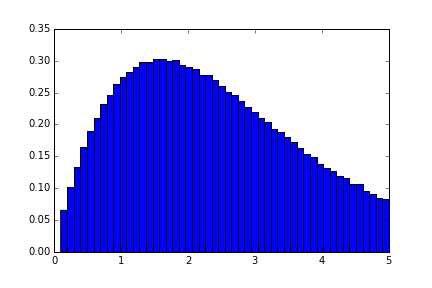
\includegraphics[]{HW1_3_6_normalized.png}
\end{figure*}
\newpage
If we simply loop over the energy domain and plot the fraction of accepted
photons in that bin then we recover $f'$.
\begin{figure*}[!h]
  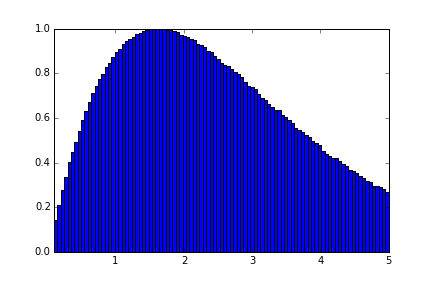
\includegraphics[]{HW1_3_6.png}
\end{figure*}
\newpage

\section*{References}
\begin{enumerate}
  \item   Matsumoto, Makoto, and Takuji Nishimura. "Mersenne Twister: A 623-dimensionally Equidistributed Uniform Pseudo-random Number Generator." Transactions on Modeling and Computer Simulation. TOMACS ACM Transactions on Modeling and Computer Simulation 8.1 (1998): 3-30.
  \item Tian, Xiang, and Khaled Benkrid. "Mersenne Twister Random Number Generation on FPGA, CPU and GPU." 2009 NASA/ESA Conference on Adaptive Hardware and Systems (2009): Web.
  \item Matsumoto, Makoto. "Mersenne Twister with Improved Initialization." Hiroshima University. Web. http://www.math.sci.hiroshima-u.ac.jp/~m-mat/MT/MT2002/emt19937ar.html.
  \item "Pseudo-Random Number Generator." Boost C++ Libraries. Web. \\ http://www.boost.org/doc/libs/1461/doc/html/boostrandom/reference.html.
  \item "Performance." Boost C++ Libraries. Web. \\ http://www.boost.org/doc/libs/1460/doc/html/boostrandom/performance.html. 
  
\end{enumerate}

\end{document}
